\section{Deep Learning Approaches for OCR}

Deep learning has fundamentally transformed Optical Character Recognition, shifting the paradigm from handcrafted feature engineering to end-to-end trainable neural architectures. Unlike traditional methods, deep learning-based OCR systems generalize across diverse scripts, fonts, and document conditions with significantly reduced reliance on domain-specific heuristics. This section surveys the major methodologies driving state-of-the-art OCR performance, tracing the progression from early convolutional approaches to modern transformer-based systems.

The foundations of deep learning in OCR were established through CNNs as feature extractors for text detection \cite{LeCun1998}. EAST proposed a direct regression pipeline predicting word-level bounding boxes in a single forward pass. CRAFT extended this by modeling character-level affinity, enabling detection of curved text, while DBNet introduced differentiable binarization to learn the detection threshold adaptively. On the recognition side, the CRNN combined CNNs with RNNs via CTC loss for direct text-line transcription without character segmentation. Attention-based models such as ASTER improved on CTC by incorporating spatial rectification, and ABINet introduced explicit bidirectional language modeling in parallel with visual decoding. Most recently, transformer architectures yielded models such as PARSeq and RT-DETR, which achieve state-of-the-art accuracy at real-time speed. Collectively, these advances reflect the replacement of modular pipelines with unified, data-driven architectures.

\subsection{CNN-based Text Detection}

CNNs enabled text detection systems to localize text regions with far greater robustness than traditional methods by learning hierarchical features directly from data. Three landmark architectures — EAST, CRAFT, and DBNet — illustrate the evolution from single-shot regression to flexible segmentation-driven approaches.

EAST marked a departure from multi-stage pipelines by proposing a fully convolutional, single-shot architecture predicting text regions at the pixel level \cite{Zhou2017}. A feature pyramid network aggregates multi-scale features, which feed two output branches: a score map for text presence and a regression branch for bounding box geometry and rotation. This streamlined design enables real-time inference on benchmarks such as ICDAR 2015 \cite{Karatzas2015}. Its primary limitation is confinement to rotated rectangles, making it unsuitable for curved or arbitrarily shaped text; performance also degrades on densely packed regions.

CRAFT addressed these limitations by shifting detection granularity to the character level \cite{Baek2019}. Rather than predicting bounding boxes directly, it produces two heat maps: a region score for character centers and an affinity score for spatial relationships between adjacent characters. Post-processing groups characters by affinity to recover text instances of arbitrary shape. A notable challenge is the absence of character-level annotations in most datasets, which the authors address via weakly supervised training with pseudo ground truth from a pretrained detector — a strategy that introduces noise and inconsistencies at character boundaries.

DBNet introduced adaptive binarization directly into the segmentation pipeline \cite{Liao2019}. Traditional approaches apply a fixed threshold to probability maps in a step decoupled from training; DBNet instead parameterizes binarization as a differentiable operation with a learned threshold map, enabling joint end-to-end optimization. This yields sharper text boundaries and better separation of closely spaced text instances, achieving strong results on curved-text benchmarks Total-Text and CTW1500. Its remaining limitation is a post-processing step requiring connected component analysis with sensitive hyperparameters.

While EAST, CRAFT, and DBNet represent substantial advances, they share a common constraint: their convolutional inductive bias limits the receptive field and makes modeling long-range spatial dependencies difficult, motivating the shift to transformer-based architectures.

\subsection{Transformer-based Text Detection and RT-DETR}

The self-attention mechanism at the core of transformers \cite{Vaswani2023} allows each position in a feature map to attend globally to all other positions, which is valuable for text detection where distant contextual cues inform local decisions. DETR \cite{Carion2020} reformulated object detection as a direct set prediction problem, removing hand-designed anchors and non-maximum suppression through bipartite matching at training time. Despite competitive accuracy, its slow convergence and insufficient inference speed limited practical deployment. Deformable DETR \cite{Zhu2021} addressed convergence by replacing dense attention with deformable attention attending to a sparse set of learned reference points, reducing complexity from quadratic to linear. DAB-DETR and DN-DETR further improved training stability, yet transformer detectors continued to lag behind CNNs in inference speed.

RT-DETR \cite{Zhao2024} resolved this bottleneck through a hybrid architecture combining convolutional efficiency with transformer expressiveness. As shown in Figure \ref{fig:rtdetr_architecture}, it consists of three components: a convolutional backbone, a hybrid encoder, and a transformer decoder with IoU-aware query selection. A pretrained backbone (e.g., ResNet) extracts multi-scale feature maps encoding both texture and semantic information.

\begin{figure}[H]
\centering
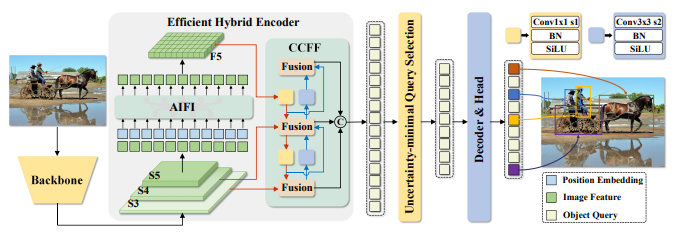
\includegraphics[width=0.8\linewidth]{images/rtdetr_architecture.png}
\caption[Overview of RT-DETR]{\textit{Overview of RT-DETR \cite{Zhao2024}}}
\label{fig:rtdetr_architecture}
\end{figure}

The hybrid encoder is RT-DETR's central innovation as illustrated in Figure \ref{fig:rtdetr_hybrid_encoder}. The Attention-based Intra-scale Feature Interaction (AIFI) module applies transformer self-attention exclusively to the highest-level feature map, where low spatial resolution makes global attention computationally feasible. The CNN-based Cross-scale Feature Fusion (CCFM) module then propagates enriched semantic context to higher-resolution maps via lightweight convolutions. This design achieves a favorable balance between representational power and inference efficiency.

\begin{figure}[ht]
\centering
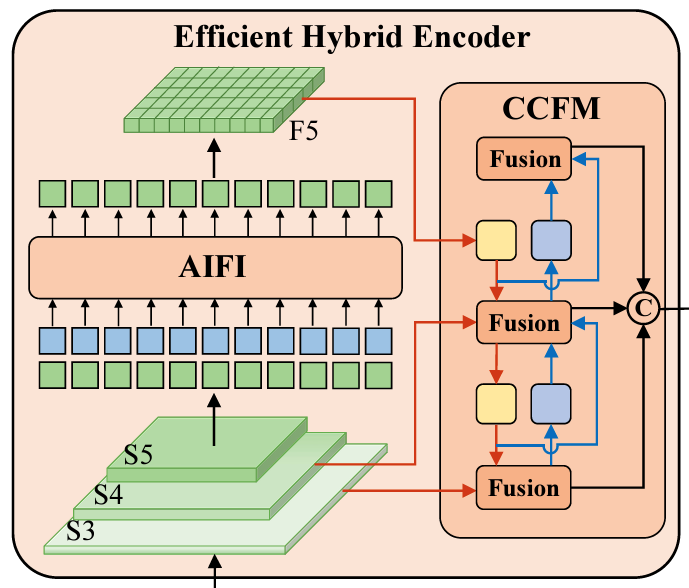
\includegraphics[width=0.6\linewidth]{images/rtdetr_hybrid_encoder.png}
\caption[Hybrid encoder of the RT-DETR model]{\textit{Hybrid encoder of the RT-DETR model \cite{Zhao2024}}}
\label{fig:rtdetr_hybrid_encoder}
\end{figure}

Query initialization is addressed through IoU-aware query selection: decoder queries are initialized from the top-scoring encoder features ranked jointly by classification confidence and predicted IoU. This yields better-calibrated initial queries than classification-only ranking, particularly for objects with high localization quality but moderate classification confidence — a common scenario in text detection.

As shown in Figure \ref{fig:rtdetr_performance}, RT-DETR with a ResNet-50 backbone achieves 53.1 AP at 108 FPS on a T4 GPU, outperforming YOLOv8-l by 1.0 AP at comparable speed. Its anchor-free design, hybrid encoder, and strong localization performance make it well-suited for Vietnamese text detection, where text lines vary considerably across document types.

\begin{figure}[ht]
\centering
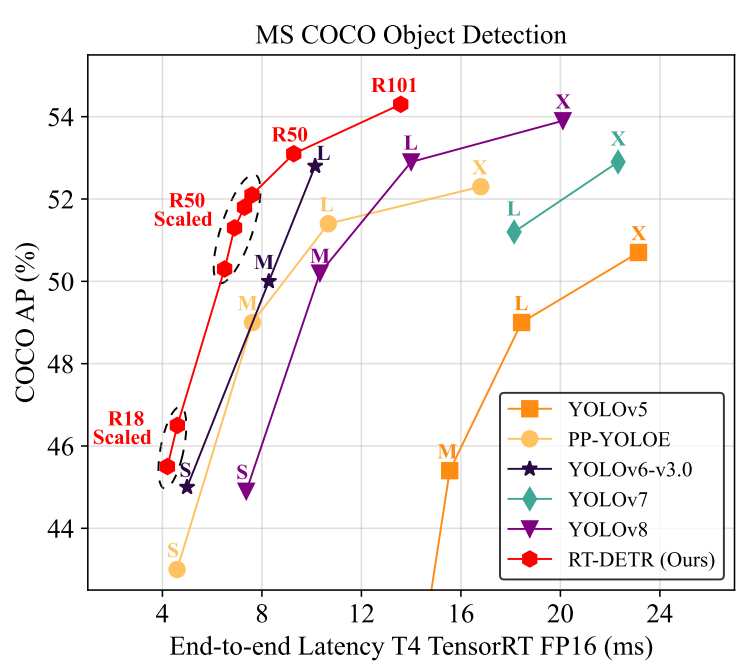
\includegraphics[width=0.6\linewidth]{images/rtdetr_performance.png}
\caption[RT-DETR latency comparison with several YOLO models]{\textit{RT-DETR latency comparison with several YOLO models \cite{Zhao2024}}}
\label{fig:rtdetr_performance}
\end{figure}

\subsection{Sequence-to-Sequence Models for Text Recognition}

Text recognition requires transcribing character sequences from images, presenting different challenges from detection. Early deep learning approaches drew from speech recognition, where recurrent architectures and probabilistic alignment had matured.

CRNN established the foundational architecture by combining a CNN feature extractor with a bidirectional LSTM, decoding output sequences via CTC loss without explicit character segmentation \cite{Shi2015}. Its simplicity and efficiency made it a widely adopted baseline. However, its recurrent bottleneck limits parallelization, and CTC's conditional independence assumption prevents explicit linguistic context modeling.

ASTER addressed geometric distortions by incorporating a learnable spatial transformer as a rectification frontend, warping the input to an approximately horizontal layout before an attention-based decoder \cite{Shi2019}. This improved accuracy on curved benchmarks such as SVT-Perspective, though the rectification adds overhead and degrades on severely distorted inputs. Attention-based encoder-decoder models more generally replaced fixed context vectors with soft alignment mechanisms, enabling selective attention to spatially relevant regions at each decoding step. AON explored multi-directional reading for irregular text, while SAR applied two-dimensional attention directly to 2D feature maps, benefiting characters with vertically complex structures.

ABINet achieved a significant conceptual advance by decoupling visual and linguistic modeling into two parallel branches \cite{Fang2021}. The visual model produces an initial prediction from image features; a separately trained bidirectional language model iteratively refines it using surrounding character context. This demonstrated that explicit linguistic modeling — rather than implicit recurrent context — is critical for high-accuracy recognition. The trade-off is added complexity from the separate language model and a more involved training process.

The progression from CRNN to ABINet reflects consistent movement toward richer contextual modeling, from local CTC decoding through soft attention to bidirectional language modeling, setting the stage for fully transformer-based recognizers.

\subsection{PARSeq and Permutation-based Recognition}

\label{sec:parseq_and_permutation_based_recognition}
PARSeq addresses limitations of prior architectures — fixed decoding orders and separately trained language models — through a unified framework combining a ViT encoder with permutation-based language modeling \cite{Bautista2022}.
The ViT encoder \cite{Dosovitskiy2021} divides the input image into a fixed grid of patches, projects each into a high-dimensional embedding, and processes all patches jointly through transformer self-attention layers. Unlike CNN encoders that aggregate context through local convolutions, the ViT captures global image structure from the first layer, relating distant character regions without deep stacking.

\begin{figure}[ht]
\centering
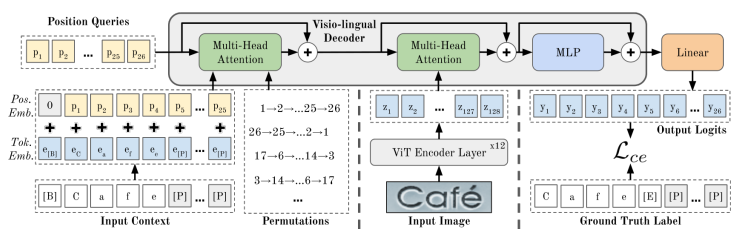
\includegraphics[width=0.8\linewidth]{images/parseq_architecture.png}
\caption[Overview of PARSeq]{\textit{Overview of PARSeq \cite{Bautista2022}}}
\label{fig:parseq_architecture}
\end{figure}

PARSeq's central innovation is its permutation-based training strategy. Rather than training the decoder in a fixed left-to-right order, PARSeq samples multiple permutations of the output sequence during training, optimizing the model to predict each character given all characters preceding it in the sampled order. This trains a single decoder to internalize all factorizations of the joint sequence probability, implicitly learning a bidirectional language model without a separate pretrained component. At inference time, an initial left-to-right pass produces a candidate sequence, which serves as context for a refinement pass correcting characters using both preceding and following context (Figure \ref{fig:parseq_permutation}). This is particularly valuable for languages with dense diacritical marks such as Vietnamese.

\begin{figure}[ht]
\centering
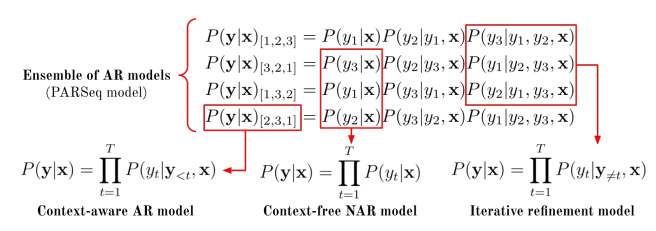
\includegraphics[width=0.8\linewidth]{images/parseq_permutation.png}
\caption[Permutation-based training strategy of PARSeq]{\textit{Permutation-based training strategy of PARSeq \cite{Bautista2022}}}
\label{fig:parseq_permutation}
\end{figure}

A further advantage is support for both autoregressive and non-autoregressive decoding within the same model, controlled by the decoder attention mask \cite{Bautista2022}. This allows practitioners to trade accuracy against speed at deployment time without retraining.

PARSeq achieved state-of-the-art accuracy across standard benchmarks (IIIT5K, SVT, ICDAR 2013/2015, SVTP, CUTE80) with a smaller parameter count than ABINet, demonstrating that permutation-based training is a more parameter-efficient mechanism for linguistic context than maintaining a separate language model. Its ViT encoder captures fine-grained spatial detail to distinguish Vietnamese diacritical marks, while its permutation-trained decoder resolves visually ambiguous characters under image degradation.

\subsection{Oriented Text Detection and Rotation-Aware Loss Functions}
\label{sec:oriented_text_detection_and_rotation_aware_loss_functions_2_2_5}

\subsubsection{Oriented Bounding Box Detection for Scene Text}
The problem of detecting arbitrarily oriented text has been an active research direction since the limitations of axis-aligned detectors became apparent on real-world scene text benchmarks. Early work on oriented text detection adapted region proposal networks to generate rotated candidate regions by augmenting the anchor parameterization with a discrete set of orientation bins. RRPN (Rotation Region Proposal Networks) \cite{Ma2018} extended the Faster RCNN framework by introducing rotation-aware anchors spanning multiple orientations and an RoI rotation pooling operation that extracts features from arbitrarily rotated candidate regions. This enabled the detector to localize text at angles not representable by axis-aligned anchors, achieving substantially improved recall on benchmarks containing multi-oriented text such as ICDAR 2015 \cite{Karatzas2015}. However, RRPN's reliance on a discrete set of predefined rotation anchors limited its angular resolution and required careful anchor design to cover the expected range of text orientations in the target domain.

TextBoxes++ \cite{Liao2018} approached the problem from a single-shot detection perspective, extending the SSD framework with irregular convolutional filters and output layers that directly regress rotated quadrilateral bounding boxes rather than axis-aligned rectangles. By predicting four corner offsets relative to a default box anchor, TextBoxes++ could represent not only rotated rectangles but also general quadrilaterals, enabling accurate enclosure of perspective-distorted text instances. This direct regression formulation avoided the angular discretization problem of anchor-based approaches but introduced training instability arising from the discontinuous nature of angular regression targets near boundary angles.

More recent work has integrated oriented detection capabilities into transformer-based frameworks, which are better suited to the anchor-free, set-prediction paradigm adopted in this thesis. Oriented RCNN \cite{Xie2021} demonstrated that a simple modification to the region proposal head, replacing axis-aligned box regression with five-parameter oriented box regression, sufficed to achieve state-of-the-art oriented detection performance without requiring specialized rotation-aware pooling operations. In the context of this work, RT-DETR is extended with an additional angle prediction head that regresses orientation as a two-dimensional unit vector in sine-cosine space, rather than as a scalar angle in degrees. This sine-cosine encoding avoids the angular discontinuity problem that arises when scalar angle regression crosses the boundary between 0 and 360 degrees, ensuring smooth and continuous gradient flow during training regardless of the predicted orientation.

\subsubsection{Gaussian Wasserstein Distance Loss for Oriented Box Regression}

A key challenge in training oriented detectors is designing a regression loss that accurately measures geometric discrepancy between predicted and ground truth OBBs. Standard IoU losses are computationally expensive and numerically unstable for rotated boxes, and yield zero gradient for non-overlapping boxes regardless of spatial proximity \cite{Yang2022}.

Yang et al. \cite{Yang2022} proposed the Gaussian Wasserstein Distance (GWD) loss by representing each oriented box as a 2D Gaussian distribution (Figure \ref{fig:gwd_gaussian}). An OBB with center $(\mu_x, \mu_y)$, half-axes $(w/2, h/2)$, and rotation $R$ maps to mean $\boldsymbol{\mu} = (\mu_x, \mu_y)$ and covariance:
\begin{equation}
\boldsymbol{\Sigma} = R \begin{pmatrix} (w/2)^2 & 0 \\ 0 & (h/2)^2 \end{pmatrix} R^\top
\end{equation}
\newpage
Geometric discrepancy is then measured as the squared Wasserstein-2 distance between corresponding Gaussians:
\begin{equation}
\text{GWD}^2(\mathcal{G}_1, \mathcal{G}_2) = |\boldsymbol{\mu}_1 - \boldsymbol{\mu}_2|^2 + \text{Tr}\left(\boldsymbol{\Sigma}_1 + \boldsymbol{\Sigma}_2 - 2\left(\boldsymbol{\Sigma}_1^{1/2} \boldsymbol{\Sigma}_2 \boldsymbol{\Sigma}_1^{1/2}\right)^{1/2}\right)
\end{equation}
The final GWD loss is defined as:
\begin{equation}
\mathcal{L}_{\text{GWD}} = 1 - \frac{1}{1 + \sqrt{\text{GWD}^2} / \tau}
\end{equation}

where $\tau$ is a scaling hyperparameter. This formulation is differentiable with respect to all box parameters, provides gradient signal even for non-overlapping boxes, and degrades gracefully under near-degenerate configurations.

\begin{figure}[H]
\centering
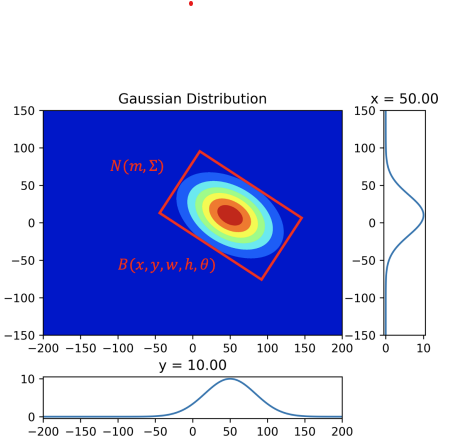
\includegraphics[width=0.6\linewidth]{images/gwd_gaussian_mapping.png}
\caption[OBB to Gaussian distribution mapping]{\textit{Equivalence between an oriented bounding box $B(x, y, w, h, \theta)$ and its 2D Gaussian $N(m, \Sigma)$ \cite{Yang2022}}}
\label{fig:gwd_gaussian}
\end{figure}

Unlike smooth-L1 loss applied per parameter, GWD treats the oriented box as a unified geometric object, penalizing deviations in all parameters jointly. This is particularly important for Vietnamese documents where text lines frequently appear at slight skew angles and regression targets for width, height, and angle are strongly correlated. The adoption of GWD loss alongside sine-cosine angle encoding and an angle-specific regression head constitutes one of the principal technical contributions of the methodology chapter.

\subsection{Vietnamese-Specific Adaptations in OCR Systems}

General-purpose OCR systems do not transfer directly to Vietnamese without targeted adaptation. Vietnamese employs a rich system of composite diacritical marks in which each syllable may carry both a vowel modification diacritic and one of six tonal markers, yielding over 130 distinct base-diacritic-tone combinations that are visually similar under low resolution or degradation \cite{QuocBinhNguyen2020}. Standard ASCII-based output vocabularies are structurally inadequate since no single ASCII character corresponds to a composite Vietnamese glyph.

Two complementary strategies address these challenges. The first is \textit{vocabulary extension}: the output projection layer of a pretrained recognizer is replaced with a larger one covering all phonologically valid composite Vietnamese glyphs, initializing shared units from pretrained weights and new units randomly, then fine-tuning on Vietnamese data. The second is \textit{class-weighted training}: cross-entropy loss weights inversely proportional to glyph frequency counteract bias toward common base characters at the expense of rare but semantically critical tone-diacritic combinations.

A further inference-stage adaptation is the \textit{phonological validity mask}, which restricts decoder outputs to character sequences that are phonologically possible in Vietnamese. Since the set of valid Vietnamese syllables is finite and rule-governed, impossible sequences (e.g., a tonal marker applied to a consonant) can be eliminated at decoding time without additional learned parameters, reducing linguistically impossible outputs under degraded image conditions. Collectively, these adaptations form the basis for the Vietnamese-specific optimization strategy applied to the recognition stage of the system developed in this thesis.
